\section*{Appendix}

The 2D environment used for this project, code found online by YouTuber "Tech with Tim"\\
https://github.com/techwithtim/Pygame-Car-Racer\\
https://www.youtube.com/playlist?list=PLzMcBGfZo4-kmY7Nh4kI9kPPnxJ5JMRPj
\begin{center}
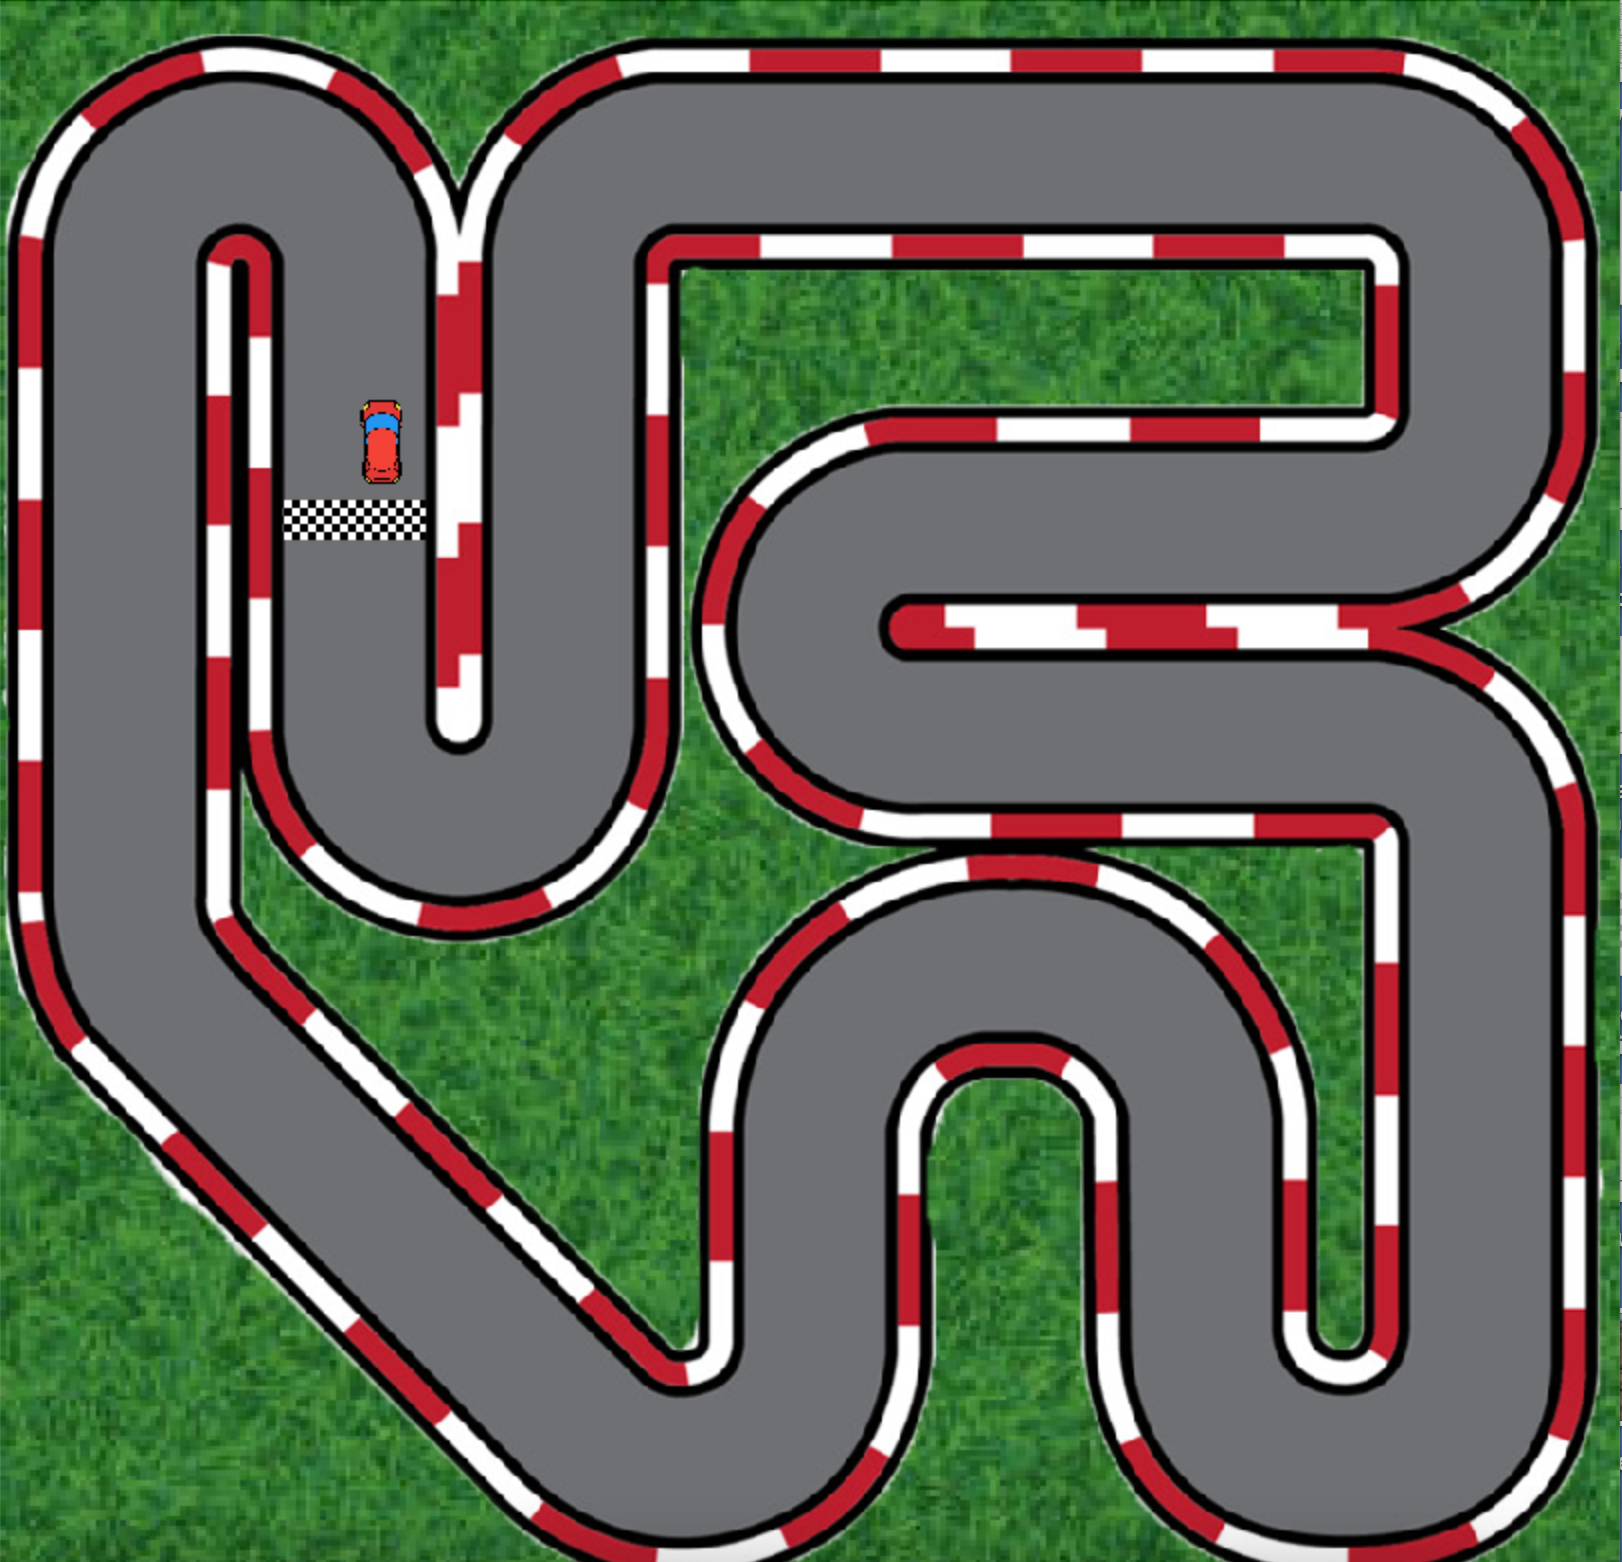
\includegraphics[scale=0.3]{Billeder/environment.png}\\
\end{center}
The reward system set up for the q-learning algorithm.
\begin{center}
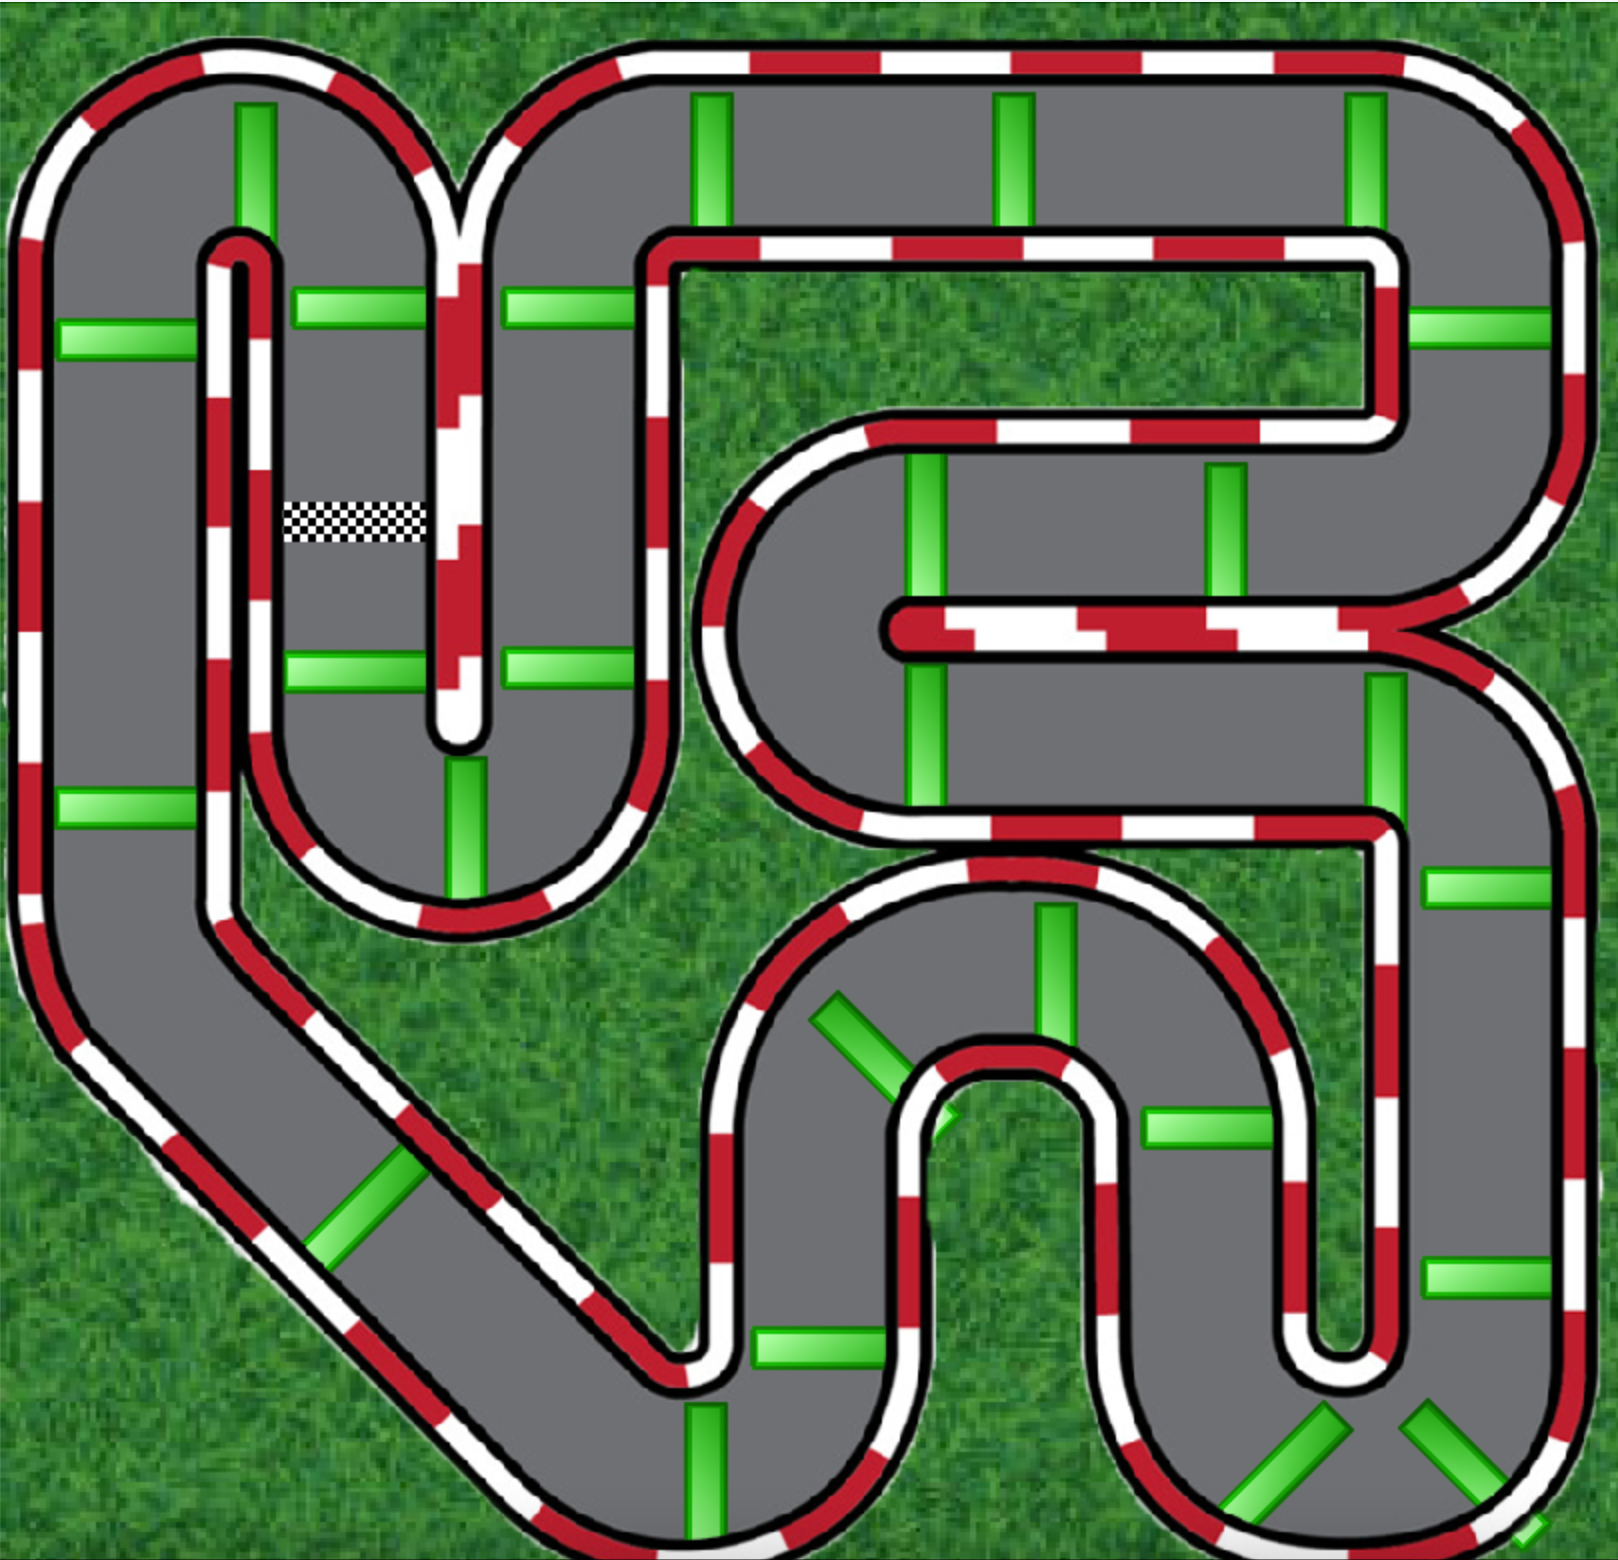
\includegraphics[scale=0.3]{Billeder/reward.png}\\
\end{center}
\newpage
The three dot-configurations. 2-point dots, cone-shaped and semicircle
\begin{center}
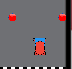
\includegraphics[scale=1]{Billeder/2-punkt.PNG} 
\hspace{0.5mm}
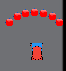
\includegraphics[svale=0.6]{Billeder/Keglesnit.PNG}
\hspace{0.5mm}
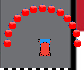
\includegraphics[svale=0.6]{Billeder/Halvcirkel.PNG}
\end{center}

